\section{Introduction}

System identification is the discipline focused on techniques for extracting models from data.
\begin{figure}[H]
    \centering
    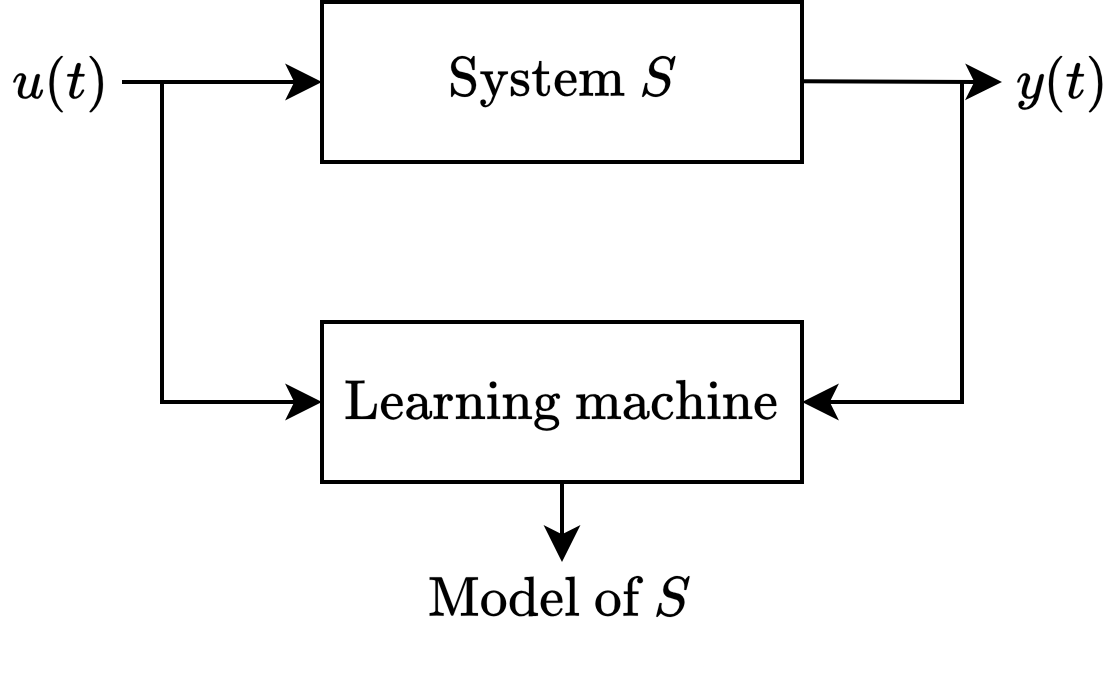
\includegraphics[width=0.6\linewidth]{images/identification.png}
    \caption{Identification process}
\end{figure}
In essence, the core components of the identification challenge include:
\begin{enumerate}
    \item The system $\mathcal{S}$. 
    \item The class of models $\mathcal{M}$. 
    \item The method of identification $\mathcal{I}$. 
    \item The experimental setup for identification $\mathcal{E}$. 
\end{enumerate}

\subsection{Parametric system identification}
The steps involved in parametric system identification are outlined below:
\begin{enumerate} 
    \item \textit{Experiment design and data collection}: the initial step involves designing experiments and gathering data. 
        Sometimes data are predefined, making it impossible to conduct further experiments. 
        In other cases, where the system is accessible, additional data can be collected. 
        In such scenarios, the choice of input signal $u(t)$ impacts the informativeness, while the data length $N$ affects the confidence level.
    \item \textit{Selection of a parametric model class} $\mathcal{M}(\vartheta)=\left\{ M(\vartheta),\vartheta \in \vartheta\right\}$: this step entails choosing a suitable parametric model class.
        Considerations include discrete or continuous time, linear or nonlinear, time-invariant or time-varying, and static or dynamic models. 
        To fully define $y(t)$ as ARMA or ARMAX process, $\vartheta$ alone isn't sufficient; parameters such as $n_a$, $n_b$, $n_c$, pure delay, and  White Noise characteristics expressed through $\lambda^2$ must also be specified.
        Notably, the pure delay and $\lambda^2$ aren't critical as they're derived from the $n$ parameters.
        Admissible values for $\vartheta$ must also be determined.
    \item \textit{Choice of the identification criterion} $J_N(\vartheta)\geq 0$: the identification criterion is chosen, often based on prediction error minimization. 
        For instance, using the predictive approach, the criterion $J_N(\vartheta)$ can be defined as the expected square prediction error:
        \[J_N(\vartheta)=\mathbb{E}\left[ \left(y(t+1)-\hat{y}(t+1\mid t)\right)^2 \right]\]
        A low prediction error indicates a good model.
        Typically, a one-step-ahead predictor is chosen for optimality checks, ensuring the prediction error equals $\lambda^2$.
        Therefore, $J_N(\hat{\vartheta}_N) \approx \lambda^2$
    \item \textit{Minimization of $J_N(\vartheta)$} with respect to $\vartheta$: this step involves minimizing the criterion function $J_N(\vartheta)$ to estimate the parameters $\hat{\vartheta}_N$.
        Depending on the model, the criterion function could be quadratic or non-quadratic.
    \item \textit{Model validation}: despite assumptions made during the process, such as the system belonging to a specific model set and fixed values for $n_a$, $n_b$, and $n_c$, it's essential to validate the model's quality. 
        This involves performing quality checks to ensure the identified model accurately represents the system dynamics.
\end{enumerate}